У даному розділі досліджено плоска статична задача теорії пружності для прямокутної області,
за умов другої основної задачі теорії пружності на бічних гранях.

Вихідна задача зведена до одновимірної задачі у просторі трансформант за допомогою інтегрального перетворення Фур'є.
Отримана крайова задача розв'язана точно за допомогою методу матрично диференціального числення,
фундаментальний розв'язок представлений як інтеграл по замкненому контору, який в свою чергу, був знайденний за допомогою теоремі про лишки.
Остаточний вигляд для функцій переміщеннь та напружень отриман шляхом оберненого перетворення Фур'є.
Побудовано та розв'язано сінгульрне інтегральне рівняння відносно невідомої функції шляхом викорстання методу ортагональних многочленів, та зведення рівнняння до бескінечної алгебричної системи,
яка в подальшому була розв'язана методом редукціі \cite{popov_3}.

Проведено чисельний аналіз отриманих функцій переміщень та напружень для різних розмірів прямокутної області та різних видів навантаження.

\subsection{Постановка задачі}
\begin{figure}[ht!]
    \begin{center}
        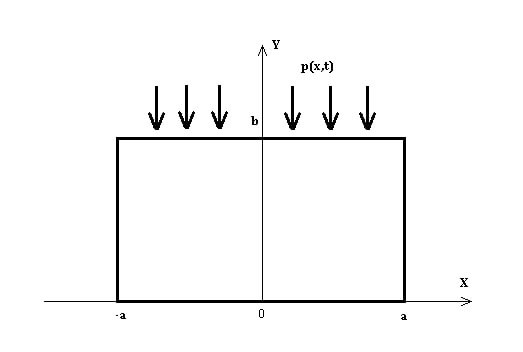
\includegraphics[scale=1]{images/geometry/image_1.jpg}
    \end{center}
    \caption{Геометрія проблеми}\label{geom_static_2}
\end{figure}
Розглядається пружна прямокутна область (Рис: \ref{geom_static_2}), яка займає облась,
що описується у декартовій системі координат співвідношенням $-a \le x \le a$, $0 \le y \le b$.

До прямокутної області на грані $y=b$ додане нормальне навантаження
\begin{equation}
    \sigma_y(x, y) |_{y=b} = -p(x), \quad  \tau_{xy}(x,y) |_{y=b} =0
\end{equation}
де $p(x)$ відома функція.

На бічних гранях виконується умова другої основної задачі теорії пружності
\begin{equation}
    u(x,y) |_{x=\pm a} = 0, \quad v(x,y) |_{x=\pm a} =0
\end{equation}
На нижній грані виконуються наступні умови
\begin{equation}
    v(x,y) |_{y=0} = 0, \quad \tau_{xy}(x,y) |_{y=0} =0
\end{equation}
Розглядаються наступні рівняння рівноваги Ламе:
\begin{equation}\label{lame_static_2}
    \begin{cases}
        \frac{\partial^2 u(x,y)}{\partial x^2} + \frac{\partial^2 u(x,y)}{\partial y^2} + \mu_0 (\frac{\partial^2 u(x,y)}{\partial x^2} + \frac{\partial^2 v(x,y)}{\partial x\partial y}) = 0 \\
        \frac{\partial^2 v(x,y)}{\partial x^2} + \frac{\partial^2 v(x,y)}{\partial y^2} + \mu_0 (\frac{\partial^2 u(x,y)}{\partial x \partial y} + \frac{\partial^2 v(x,y)}{\partial y^2}) = 0 \\
    \end{cases}
\end{equation}
Щоб розв'язати поставлену задачу буде розглянута тільки половона прямокутної області $0 \le x \le a$, $0 \le y \le b$
та використовуючи властивості симметрії граничні умови на бічних гранях будуть мати вигляд:
\begin{equation}\label{bound_1_static_2}
    u(x,y) |_{x=0} = 0, \quad \tau_{xy}(x,y) |_{x=0} =0
\end{equation}
\begin{equation}\label{bound_2_static_2}
    u(x,y) |_{x=a} = 0, \quad v(x,y) |_{x=a} = 0
\end{equation}

\subsection{Зведеня задачі до одновимірної у просторі трансформант}
Для того, щоб звести задачу до одновимірної задачі, використаєм інтегральне перетворення Фур'є по змінній $x$ у до рівнянь (\ref{lame_static_2}) наступному вигляді:
\begin{equation}
    \begin{pmatrix}
        u_n(y) \\
        v_n(y)
    \end{pmatrix} = \int_{0}^{a} 
    \begin{pmatrix}
        u(x,y) sin(\alpha_n x) \\
        v(x,y) cos(\alpha_n x)
    \end{pmatrix} dx, \quad \alpha_n = \frac{\pi n}{a}
\end{equation}

Для цього помножим перше та друге рівняння (\ref{lame_static_2}) на $sin(\alpha_n x)$ та $cos(\alpha_n x)$ відповідно та проінтегруєм по змінній $x$ на інтервалі $0 \le x \le a$.
Покрокове інтегрування рівняння (\ref{lame_static_2}) наведено у (\nameref{ap_A}).
Отримана система рівнянь задачі у просторі трансформант:
\begin{equation}\label{transf_static_2}
    \begin{cases}
        u_n^{''}(y) - \alpha_n \mu_0 v_n^{'}(y) - \alpha_n^2 (1 + \mu_0) u_n(y) = 0 \\
        (1 + \mu_0) v_n^{''}(y) + \alpha_n \mu_0 u_n^{'}(y)  - \alpha_n^2 v_n(y) = -cos(\alpha_n) f(y) \\
    \end{cases}
\end{equation}
Де $f(y) = \frac{\partial v(x,y)}{\partial x}|_{x=a}$ - невідома функція

Застосовуючи інтегральне перетворення до граничних умов,
отримаємо наступні умови задачі у просторі трансформант
\begin{equation}\label{transf_bound_static_2}
    \begin{cases}
        \left( (2G + \lambda)v_n^{'}(y) + \alpha_n \lambda u_n(y) \right)|_{y=b} = -p_n \\
        \left(u_n^{'}(y) - \alpha_n v_n(y)  \right)|_{y=b} = 0 \\
        v_n(y)|_{y=0} = 0 \\
        \left(u_n^{'}(y) - \alpha_n v_n(y)  \right)|_{y=0} = 0
    \end{cases}
\end{equation}
Де $p_n = \int_{0}^{a} p(x) cos(\alpha_n x) dx$

\subsection{Зведення задачі у просторі трансформант до матрично-векторної форми}
Для того щоб розв'язати задачу у простосторі трансформант, перепишмо її у матрично-векторній формі.
Рівняння рівноваги (\ref{transf_static_2}) запишемо у наступному вигляді:
\begin{align}\label{transf_mat_static_2}
    &L_2\left[ Z_n(y) \right] = A * Z_n^{''}(y) + B * Z_n^{'}(y) + C * Z_n(y) \nonumber \\
    &L_2\left[ Z_n(y) \right] = F_n(y)
\end{align}
Де
\begin{equation*}
    A = \begin{pmatrix}
        1 & 0 \\
        0 & 1 + \mu_0
    \end{pmatrix}, \quad
    B = \begin{pmatrix}
        0 & -\alpha_n \mu_0 \\
        \alpha_n \mu_0 & 0
    \end{pmatrix}, \quad
    C = \begin{pmatrix}
        -\alpha_n^2(1 + \mu_0) & 0 \\
        0 & -\alpha_n^2
    \end{pmatrix}
\end{equation*}
\begin{equation*}
    Z_n(y) = \begin{pmatrix}
        u_n(y) \\
        v_n(y)
    \end{pmatrix}, \quad 
    F_n(y) = \begin{pmatrix}
        0 \\
        - cos(\alpha_n a) f(y)
    \end{pmatrix}
\end{equation*}
Граничні умови (\ref{transf_bound_static_2}) запишемо у наступному вигляді:
\begin{align}\label{transf_bound_mat_static_2}
    &U_i\left[ Z_n(y) \right] = E_i * Z_n^{'}(b_i) + F_i * Z_n(b_i) \nonumber \\
    & U_i\left[ Z_n(y) \right] = D_i
\end{align}
Де $i = \overline{0, 1}$, $b_0 = b$, $b_1 = 0$,
\begin{equation*}
    E_0 = \begin{pmatrix}
        1 & 0 \\
        0 & 2G + \lambda
    \end{pmatrix}, \quad
    F_0 = \begin{pmatrix}
        0 & -\alpha_n \\
        \alpha_n \lambda & 0
    \end{pmatrix}, \quad
\end{equation*}
\begin{equation*}
    E_1 = \begin{pmatrix}
        1 & 0 \\
        0 & 0
    \end{pmatrix}, \quad
    F_1 = \begin{pmatrix}
        0 & -\alpha_n \\
        0 & 1
    \end{pmatrix}, \quad
\end{equation*}
\begin{equation*}
    D_0 = \begin{pmatrix}
        0 \\
        -p_n
    \end{pmatrix}, \quad
    D_1 = \begin{pmatrix}
        0 \\
        0
    \end{pmatrix}, \quad
\end{equation*}

Для знаходження розв'язку задачі у просторі трансформант, знайдем фундаментальну матрицю рівняння (\ref{transf_mat_static_2}).
Шукати її будем у наступному вигляді \cite{gantmaher}:
\begin{equation}
    Y(y) = \frac{1}{2\pi i} \oint_C e^{sy} M^{-1}(s)ds
\end{equation}
Де $M(s)$ - характерестична матриця рівняння (\ref{transf_mat_static_2}), а $C$ - замкнений контур який містить усі особливі точки. Яку будемо шукати з наступної умовни
\begin{equation}
    L_2\left[ e^{sy}*I \right] = e^{sy} * M(s), \quad I = \begin{pmatrix} 1 & 0 \\ 0 & 1 \end{pmatrix}
\end{equation}
\begin{align*}
    &L_2\left[ e^{sy}*I \right] = e^{sy} \left( s^2A * I + s B*I + C*I \right) = \\
    &=e^{sy} \left( \begin{pmatrix}
        s^2 & 0 \\
        0 & s^2 (1 + \mu_0)
    \end{pmatrix} + \begin{pmatrix}
        0 & -\alpha_n \mu_0 s\\
        \alpha_n \mu_0 s & 0
    \end{pmatrix} + \begin{pmatrix}
        -\alpha_n^2(1 + \mu_0) & 0 \\
        0 & -\alpha_n^2
    \end{pmatrix} \right) =  \\
    &=e^{sy} \begin{pmatrix}
        s^2 -\alpha_n^2(1 + \mu_0) & -\alpha_n \mu_0 s \\
        \alpha_n \mu_0 s & s^2 (1 + \mu_0) -\alpha_n^2
     \end{pmatrix} =>
\end{align*}

\begin{equation}
    M(s) = \begin{pmatrix}
        s^2 -\alpha_n^2(1 + \mu_0) & -\alpha_n \mu_0 s \\
        \alpha_n \mu_0 s & s^2 (1 + \mu_0) -\alpha_n^2
     \end{pmatrix}
\end{equation}

Знайдемо тепер $M^{-1}(s) = \frac{\widetilde{M(s)}}{det[M(s)]}$.
\begin{equation}
    \widetilde{M(s)} = \begin{pmatrix}
        s^2 (1 + \mu_0) -\alpha_n^2 & \alpha_n \mu_0 s \\
        -\alpha_n \mu_0 s & s^2 -\alpha_n^2(1 + \mu_0)
     \end{pmatrix}
\end{equation}
\begin{align}
    &det[M(s)] = \begin{vmatrix}
        s^2 - \alpha_n^2 - \alpha_n^2\mu_0 & -\alpha_n \mu_0 s \\
        \alpha_n \mu_0 s & s^2 (1 + \mu_0) -\alpha_n^2
     \end{vmatrix} = \nonumber \\
    &=(1+\mu_0)(s - \alpha_n)^2(s + \alpha_n)^2
\end{align}
Де $\alpha_n$, $-\alpha_n$, корені $det[M(s)]=0$, детальне знаходження яких наведено в (\nameref{ap_B}).

Враховучи це, тепер знайдемо значення фундаментальної матрицю за допомогою теореми про лишки:
\begin{align*}
    &\frac{1}{2\pi i} \oint_C e^{sy} M^{-1}(s)ds = \frac{2 \pi i}{2 \pi i (1 + \mu_0)} \sum_{i=1}^{2} Res\left[ e^{sy} \frac{\widetilde{M(s)}}{det[M(s)]} \right] = \\
    & = \frac{1}{(1 + \mu_0)} \left(Y_0(y) + Y_1(y) \right)
\end{align*}
Знайдем $Y_0(y)$:
\begin{align}
    &Y_0(y) =  \frac{\partial}{\partial s} \left( \frac{e^{sy}}{(s+\alpha_n)^2} \widetilde{M(s)} \right) \Big|_{s=\alpha_n} = \nonumber \\
    &=\frac{e^{\alpha_n y}}{4\alpha_n} \begin{pmatrix}
    \alpha_n \mu_0 y + 2 + \mu_0 & \alpha_n \mu_0 y \\
    -\alpha_n \mu_0 y & -\alpha_n \mu_0 y + 2 + \mu_0
    \end{pmatrix}
\end{align}
Знайдем $Y_1(y)$:
\begin{align}
    &Y_1(y) = \frac{\partial}{\partial s} \left(\frac{e^{sy}}{(s-\alpha_n)^2} \widetilde{M(s)} \right) \Big|_{s=-\alpha_n} = \nonumber \\
    =&\frac{e^{-\alpha_n y}}{4\alpha_n} \begin{pmatrix}
    \alpha_n \mu_0 y - 2 - \mu_0 & -\alpha_n \mu_0 y \\
    \alpha_n \mu_0 y & -\alpha_n \mu_0 y - 2 - \mu_0
    \end{pmatrix}
\end{align}

\subsection{Побудова матриці-функції Гріна}
Для побудови матриці-функції Гріна спочатку знайдем тепер фундамельні бизисні матриці $\Psi_0(y)$, $\Psi_1(y)$, шукати їх будем у наступному вигляді:
\begin{equation}\label{psi_static_2}
    \Psi_i(y) = Y_0(y) * C_1^i + Y_2(y) * C_2^i
\end{equation}

Залишилось знайти невідомі матриці коєфіцієнтів $C_1^0$, $C_2^0$, $C_1^1$, $C_2^1$ використовуючи граничні умови \eqref{transf_bound_mat_static_2}.
Покрокове знаходження яких наведено у (\nameref{ap_C}).
Для подальшого введемо наступні позначення для елементів матриць $\Psi_0(y)$, $\Psi_1(y)$:
\begin{equation*}
    \Psi_0(y) = \begin{pmatrix}
        \Psi_1^0(y) &  \Psi_2^0(y) \\
        \Psi_3^0(y) &  \Psi_4^0(y) 
    \end{pmatrix}, \quad 
    \Psi_1(y) = \begin{pmatrix}
        \Psi_1^1(y) &  \Psi_2^1(y) \\
        \Psi_3^1(y) &  \Psi_4^1(y) 
    \end{pmatrix}      
\end{equation*}

Таким чином матрицю Гріна можемо записати у вигляді:
\begin{equation}
    G(y,\xi) = 
    \begin{cases}
        \Psi_0(y) * \Psi_1(\xi), \quad 0 \le y < \xi \\
        \Psi_1(y) * \Psi_0(\xi), \quad \xi < y \le b
    \end{cases}
\end{equation}

Для данної матриці Гріна виконано усі властивості, зокрема виконані однорідні граничні умови \eqref{transf_bound_mat_static_2}
та однорідні рівняння рівноваги у просторі трансформант \eqref{transf_mat_static_2}:
\begin{equation*}
    L_2\left[  G(y, \xi) \right] = 0
\end{equation*}
\begin{equation*}
    U_0\left[ G(y, \xi) \right] = 0, \quad  U_1\left[ G(y, \xi) \right],
\end{equation*}

Таким чином ми можемо записати розв'язок крайової задачі у просторі трансформант:
\begin{equation}
    Z_n(y) = \int_0^b G(y,\xi) F_n(\xi) d\xi + \Psi_0(y) * D_0 + \Psi_1(y) * D_1
\end{equation}

Введемо наступні позначення $G(y, \xi) = \begin{pmatrix}
    g_1(y,\xi) & g_2(y,\xi) \\
    g_3(y,\xi) & g_4(y,\xi)
\end{pmatrix}$, $F_n(y) = \begin{pmatrix}
    f_n^1(y) \\
    f_n^2(y)
\end{pmatrix}$, $\Psi_i(y) = \begin{pmatrix}
    \psi_i^1(y) & \psi_i^2(y) \\
    \psi_i^3(y) & \psi_i^4(y)
\end{pmatrix}$, $i=0,1$. Враховуючи це, шукані функціі перемішень у просторі трансформант можна записати у наступному вигляді
\begin{align}\label{transf_sol_u_static_2}
    &u_n(y) = \int_0^b \left[g_1(y, \xi)f_n^1(\xi) + g_2(y, \xi)f_n^2(\xi) \right]d\xi - \psi_0^2(y) p_n
\end{align}
\begin{align}\label{transf_sol_v_static_2}
    &v_n(y) = \int_0^b \left[g_3(y, \xi)f_n^1(\xi) + g_4(y, \xi)f_n^2(\xi) \right]d\xi - \psi_0^4(y) p_n
\end{align}

\subsection{Побудова розв'язоку вихідної задачі}
Викорустовуючи обернене інтегральне перетворення Фур'є до розв'язку задачі у просторі трансформант
(\ref{transf_sol_u_static_2}), (\ref{transf_sol_u_static_2}), отримаємо фінальний розв'язок задачі
\begin{equation}
    u(x,y) = \frac{2}{a} \sum_{n=1}^{\infty} u_n(y) sin(\alpha_n x), \quad \alpha_n = \frac{\pi n}{a}
\end{equation}
\begin{equation}
    v(x,y) = \frac{v_0(y)}{a} + \frac{2}{a} \sum_{n=1}^{\infty} v_n(y) cos(\alpha_n x), \quad \alpha_n = \frac{\pi n}{a}
\end{equation}

Знайдем тепер $v_0(y)$ розглянувши задачу у просторі трансформант \eqref{transf_static_2}, \eqref{transf_bound_static_2} при $n=0$, $\alpha_n = 0$.
Детальний розв'язок якої наведено в (\nameref{ap_D}). Тоді остаточний розв'язок $v(x,y)$ буде мати вигляд
\begin{align}
    &v(x,y) = \frac{2}{a} \sum_{n=1}^{\infty} v_n(y) cos(\alpha_n x) - \frac{p_0}{a(2G + \lambda)} - \\
    &- \frac{1}{a(1+\mu_0)} \int_{0}^{b}g(y,\xi) f(\xi) d\xi
\end{align}

\subsection{Розв'язок сінгулярного інтегрального рівняння}
Залишилось знайти невідому функцію $f(y)$ для якої побудуєм інтегральне рівнняння використовуючи граничну умову $\sigma_y(x, y) |_{y=b} = -p(x)$.
\begin{equation*}
    (2G + \lambda)\frac{\partial v(x,y)}{\partial y}|_{y=b} + \lambda\frac{\partial u(x,y)}{\partial x}|_{y=b} = -p(x) \Leftrightarrow
\end{equation*}
\begin{align*}
    &-\frac{(2G + \lambda)}{a(1+\mu_0)} \int_{0}^{b}\frac{\partial g(y, \xi)}{\partial y}|_{y=b} f(\xi) d\xi - \\
    &- \frac{2(2G + \lambda)}{a} \frac{\partial}{\partial y} \sum_{n=1}^{\infty} \left( \int_0^b \left[g_4(y, \xi) cos(\alpha_n a) f(\xi) \right]d\xi + \psi_0^{4}(y) p_n \right) \\ 
    &cos(\alpha_n x)|_{y=b} -\frac{2\lambda}{a} \frac{\partial}{\partial x} \sum_{n=1}^{\infty} \left( \int_0^b \left[g_2(y, \xi)cos(\alpha_n a) f(\xi) \right]d\xi + \psi_0^2(y) p_n \right) \\
    &sin(\alpha_n x)|_{y=b} = -p(x)
\end{align*}
Введемо позначення:
\begin{align}
    &a_1(x) = a p(x) - 2(2G + \lambda) \frac{\partial}{\partial y} \sum_{n=1}^{\infty} \psi_0^{4}(y) p_n cos(\alpha_n x)|_{y=b} - \nonumber \\
    &- 2\lambda \frac{\partial}{\partial x} \sum_{n=1}^{\infty}\psi_0^2(y) p_n sin(\alpha_n x)|_{y=b}
\end{align}
Враховуючи його отримаємо наступне інтегральне рівняння відносно $f(\xi)$:
\begin{align}\label{int_static_2}
    &\frac{(2G + \lambda)}{(1+\mu_0)} \int_{0}^{b}\frac{\partial g(y, \xi)}{\partial y}|_{y=b} f(\xi) d\xi + \nonumber \\ 
    &+ \int_{0}^{b} \sum_{n=1}^{\infty} cos(\alpha_n a) cos(\alpha_n x) \left[(2G + \lambda) \frac{\partial g_4(y, \xi)}{\partial y} + \alpha_n \lambda g_2(y, \xi) \right]|_{y=b} \nonumber \\ 
    &f(\xi) d\xi = a_1(x)
\end{align}
Розглянемо ряд:
\begin{align*}
    &\sum_{n=1}^{\infty} cos(\alpha_n a) cos(\alpha_n x) \left[(2G + \lambda) \frac{\partial g_4(y, \xi)}{\partial y} + \alpha_n \lambda g_2(y, \xi) \right]|_{y=b} = \\
    &= \sum_{n=1}^{\infty} (-1)^n \alpha_n^{-1} e^{\alpha_n (\xi - b)} cos(\alpha_n x) \left[ \frac{\partial \widetilde{g_4(y, \xi)}}{\partial y} + \lambda \widetilde{g_2(y, \xi)} \right]|_{y=b} = \\
    &= \sum_{n=1}^{N} (-1)^n \alpha_n^{-1} e^{\alpha_n (\xi - b)} cos(\alpha_n x) \left[ \frac{\partial \widetilde{g_4(y, \xi)}}{\partial y} + \lambda \widetilde{g_2(y, \xi)} \right]|_{y=b} + \\
    & + a_2 \sum_{n=N}^{\infty} (-1)^n (2n + 1)^{-1} e^{-(2n + 1) \frac{\pi}{2a} (b - \xi)} cos((2n + 1) \frac{\pi}{2a} x) + \\
    & + a_2 \sum_{n=0}^{N} (-1)^n (2n + 1)^{-1} e^{-(2n + 1) \frac{\pi}{2a} (b - \xi)} cos((2n + 1) \frac{\pi}{2a} x) - \\
    & - a_2 \sum_{n=0}^{N} (-1)^n (2n + 1)^{-1} e^{-(2n + 1) \frac{\pi}{2a} (b - \xi)} cos((2n + 1) \frac{\pi}{2a} x) = \\
    &= a_2 \sum_{n=0}^{\infty} (-1)^n (2n + 1)^{-1} e^{-(2n + 1) \frac{\pi}{2a} (b - \xi)} cos((2n + 1) \frac{\pi}{2a} x) + a_3(\xi, x)
\end{align*}

Використовуючи формулу 5.4.12.8 \cite{prudnikov} отримаємо:
\begin{align*}
    &a_2 \sum_{n=0}^{\infty} (-1)^n (2n + 1)^{-1} e^{-(2n + 1) \frac{\pi}{2a} (b - \xi)} cos((2n + 1) \frac{\pi}{2a} x) + a_3(\xi, x) = \\
    &= \frac{a_2}{4} ln\left[ \frac{ch(\frac{\pi}{2a}(b - \xi)) + cos(\frac{\pi}{2a}x)}{ch(\frac{\pi}{2a}(b - \xi)) - cos(\frac{\pi}{2a}x)} \right] + a_3(\xi, x)
\end{align*}

Де:
\begin{equation*}
    a_2 = \frac{2}{\pi} \lim_{n \rightarrow \infty}\left[ \frac{\partial \widetilde{g_4(y, \xi)}}{\partial y} + \lambda \widetilde{g_2(y, \xi)} \right]|_{y=b}, 
\end{equation*}
\begin{align*}
    &a_3(\xi, x) = \sum_{n=1}^{N} cos(\alpha_n a) cos(\alpha_n x) \left[(2G + \lambda) \frac{\partial g_4(y, \xi)}{\partial y} + \alpha_n \lambda g_2(y, \xi) \right]|_{y=b} - \\
    & - a_2 \sum_{n=0}^{N} (-1)^n (2n + 1)^{-1} e^{-(2n + 1) \frac{\pi}{2a} (b - \xi)} cos((2n + 1) \frac{\pi}{2a} x)
\end{align*}

Повернемося до інтегралу
\begin{align}
    &\frac{(2G + \lambda)}{(1+\mu_0)} \int_{0}^{b}\frac{\partial g(y, \xi)}{\partial y}|_{y=b} f(\xi) d\xi + \int_{0}^{b} \left( \frac{a_2}{4} ln\left[ \frac{ch(\frac{\pi}{2a}(b - \xi)) + cos(\frac{\pi}{2a}x)}{ch(\frac{\pi}{2a}(b - \xi)) - cos(\frac{\pi}{2a}x)} \right] + a_3(\xi, x) \right) f(\xi) d\xi = \\
    & = \int_{0}^{b} \left( \frac{a_2}{4} ln\left[ \frac{ch(\frac{\pi}{2a}(b - \xi)) + cos(\frac{\pi}{2a}x)}{ch(\frac{\pi}{2a}(b - \xi)) - cos(\frac{\pi}{2a}x)} \right] + a_3(\xi, x) + \frac{(2G + \lambda)}{(1+\mu_0)} \frac{\partial g(y, \xi)}{\partial y}|_{y=b} \right) f(\xi) d\xi = \\
    &= \left[
        \begin{matrix}
            t = \frac{ch(\frac{\pi}{2a}(b - \xi)) - 1}{1 - ch(\frac{\pi b}{2a})} \\
            sh(\frac{\pi}{2a}(b - \xi))d\xi = -\frac{2a}{\pi} (ch(\frac{\pi b}{2a}) - 1) dt \\
            \xi = 0, \quad t = 1 \\
            \xi = b, \quad t = 0 \\
            \xi = b - \frac{2a}{\pi} arch((ch(\frac{\pi b}{2a}) - 1)t + 1)
        \end{matrix}
        \right] = \\
    &=a_5 \int_{0}^{b} a_4(t) \left( \frac{a_2}{4} ln\left[ \frac{t + cos(\frac{\pi}{2a}x)}{t - cos(\frac{\pi}{2a}x)} \right] + \widetilde{a_3(t, x)} \right) \widetilde{f(t)} dt
\end{align}
Де:
\begin{align*}
    &\widetilde{a_3(t, x)} = a_3\left(b - \frac{2a}{\pi} arch((ch(\frac{\pi b}{2a}) - 1)t + 1), x \right) + \frac{(2G + \lambda)}{(1+\mu_0)} \frac{\partial g(y, b - \frac{2a}{\pi} arch((ch(\frac{\pi b}{2a}) - 1)t + 1))}{\partial y}|_{y=b} \\
    &f(t) = f(b - \frac{2a}{\pi} arch((ch(\frac{\pi b}{2a}) - 1)t + 1)) \\
    &a_4(t) = \frac{1}{ sh\left(arch\left[ (ch(\frac{\pi b}{2a}) - 1)t + 1 \right]\right) } \\
    &a_5 = \frac{2a}{\pi} (ch(\frac{\pi b}{2a}) - 1)
\end{align*}

Таким чином отримаємо наступне інтегральне рівняння:
\begin{equation}
    a_5 \int_{0}^{b} a_4(t) \left( \frac{a_2}{4} ln\left[ \frac{t + cos(\frac{\pi}{2a}x)}{t - cos(\frac{\pi}{2a}x)} \right] + \widetilde{a_3(t, x)} \right) \widetilde{f(t)} dt = a_1(x)
\end{equation}

Розв'язок якого будемо шукати у наступному вигляді:
\begin{equation}
    \widetilde{f(t)} = \frac{1}{a_2 a_4(t)} \frac{1}{\sqrt{1 - t^2}} \sum_{k=0}^{\infty} \varphi_k T_{2k + 1}(t) 
\end{equation}
Де $\varphi_k$ - невідомі коєфіцієнти, $T_{2k + 1}(t)$ - поліном Чебишева першого роду.

Таким чином отримаємо
\begin{align*}
    & \sum_{k=0}^{\infty}  \frac{\varphi_k}{4} \frac{1}{\pi} \int_{0}^{1} ln\left[ \frac{t + cos(\frac{\pi}{2a}x)}{t - cos(\frac{\pi}{2a}x)} \right] \frac{T_{2k + 1}(t)}{\sqrt{1 - t^2}} dt + \\
    & + \sum_{k=0}^{\infty} \varphi_k \frac{1}{\pi} \int_{0}^{1} \frac{\widetilde{a_3(t, x)}}{a_2} \frac{T_{2k + 1}(t)}{\sqrt{1 - t^2}} dt = \frac{a_1(x)}{a_5} \Leftrightarrow
\end{align*}
Використовуючи формулу B.1.9 \cite{ortogonal}
\begin{equation}\label{int_2_static_2}
    \sum_{k=0}^{\infty}  \varphi_k \frac{T_{2k + 1}( cos(\frac{\pi}{2a}x) )}{4(2k + 1)} + \sum_{k=0}^{\infty} \varphi_k \frac{1}{\pi} \int_{0}^{1} \frac{\widetilde{a_3(t, x)}}{a_2} \frac{T_{2k + 1}(t)}{\sqrt{1 - t^2}} dt = \frac{a_1(x)}{a_5}
\end{equation}

Введем позначення
\begin{equation*}
    l = cos(\frac{\pi}{2a}x), \quad \widetilde{a_1(l)} = \frac{a_1(\frac{2a}{\pi} arccos(l))}{a_5}
\end{equation*}
Помножимо обидві частини рівняння \eqref{int_2_static_2} скалярно на $\frac{T_{2m + 1}(l)}{\sqrt{1 - l^2}}$ та проінтегруєм по змінній $l$ на інтервалі $(-1; 1)$.
Та використовуючи формулу 2.3.2 \cite{ortogonal} отримаєм наступне бескінечну алгебричну систему відносно невідомих коєфіцієнтів $\varphi_k$, яка в подальшому буде розв'язуватись методом редукції.
\begin{equation}\label{int_system_gen_static_2}
    \frac{\phi_m \pi}{8(2m + 1)} + \sum_{k=0}^{\infty} \phi_k g_{k, m} = f_m
\end{equation}
Де $g_{k, m} = \frac{1}{\pi} \int_{-1}^{1} \frac{T_{2m + 1}(l)}{\sqrt{1 - l^2}} \int_{0}^{1} \frac{\widetilde{a_3(t, \frac{2a}{\pi} arccos(l) )}}{a_2} \frac{T_{2k + 1}(t)}{\sqrt{1 - t^2}} dt dl$,
$f_m = \int_{-1}^{1} \frac{T_{2m + 1}(l) \widetilde{a_1(l)}}{\sqrt{1 - l^2}} dl$ інтеграли відомих функцій

\subsection{Чисельні розрахунки}
Наведені чисельні експеренти розглядаються для сталі ($E=200$ ГПА, $\mu=0.25$).

Розглянута прямокунта область $0 \le x \le 10$, $0 \le y \le 15$, при функції навантаження $p(x)=(x-2.5)^2$.
На малюнках (Рис: \ref{static_2_u_1}), (Рис: \ref{static_2_v_1}), (Рис: \ref{static_2_sigma_x_1}), (Рис: \ref{static_2_sigma_y_1})
представлені функіі переміщень $u(x,y)$, $v(x,y)$ та напружень $\sigma_x(x,y)$, $\sigma_y(x,y)$ відповідно.
\begin{figure}[h!]
    \begin{center}
        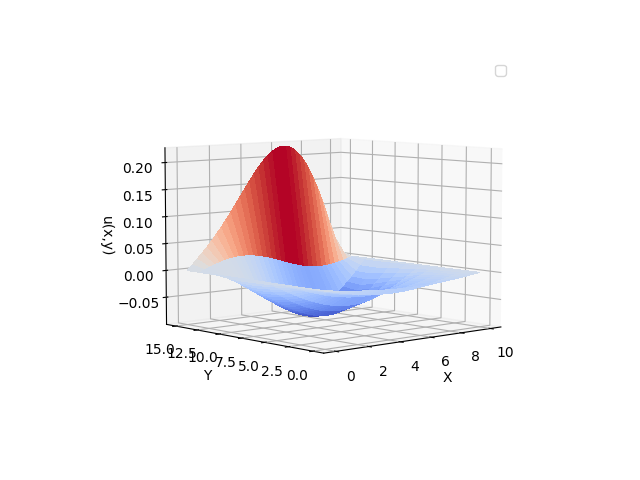
\includegraphics[width=0.49\textwidth, scale=1]{images/results/static_2/u_1.png}
        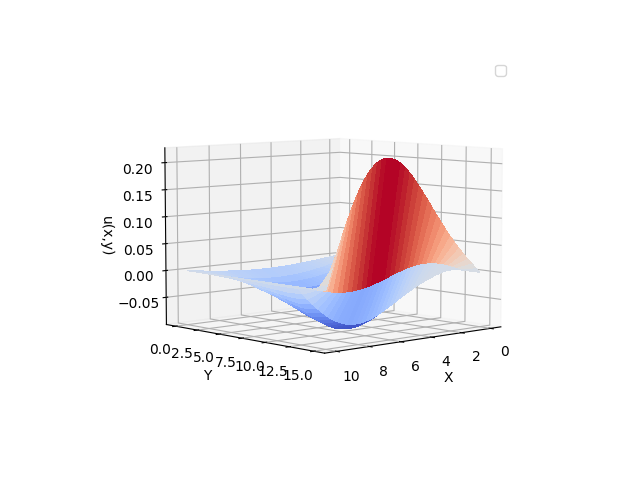
\includegraphics[width=0.49\textwidth, scale=1]{images/results/static_2/u_2.png}
        \caption{Функція $u(x, y)$}\label{static_2_u_1}
    \end{center}
\end{figure}
\newpage
\begin{figure}[h!]
    \begin{center}
        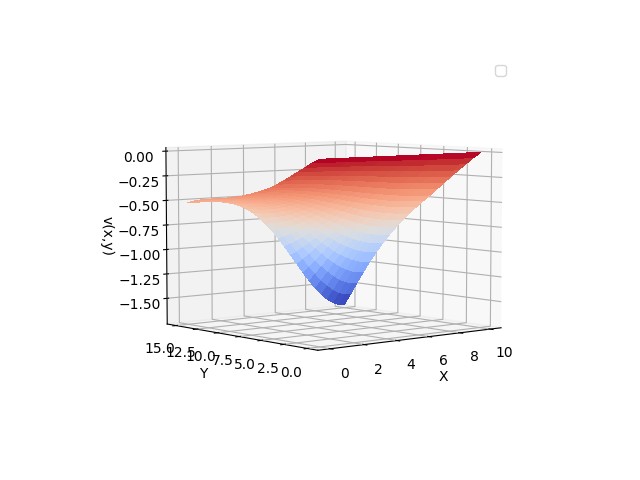
\includegraphics[width=0.49\textwidth, scale=1]{images/results/static_2/v_1.png}
        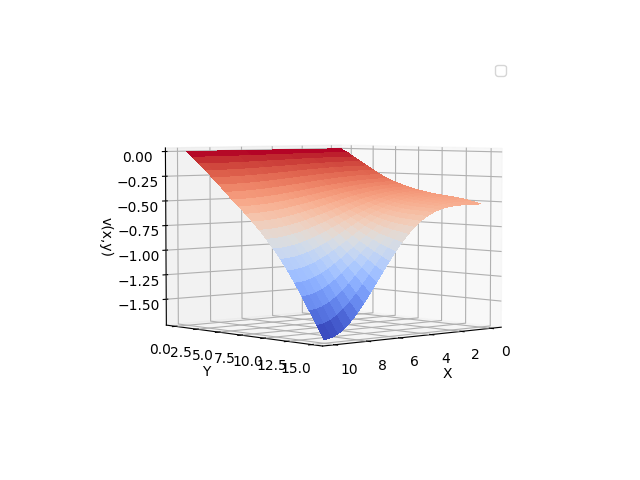
\includegraphics[width=0.49\textwidth, scale=1]{images/results/static_2/v_2.png}
        \caption{Функція $v(x, y)$}\label{static_2_v_1}
    \end{center}
\end{figure}
\begin{figure}[h!]
    \begin{center}
        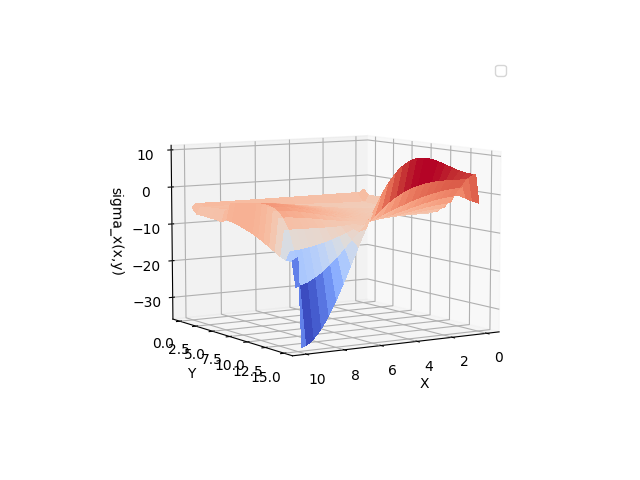
\includegraphics[width=0.49\textwidth, scale=1]{images/results/static_2/sigma_x_1.png}
        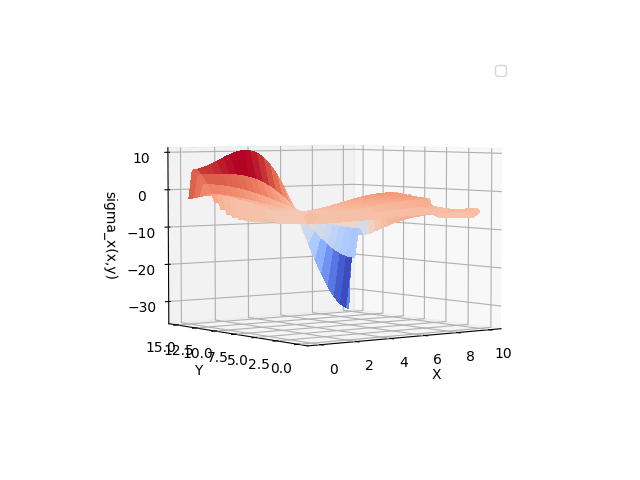
\includegraphics[width=0.49\textwidth, scale=1]{images/results/static_2/sigma_x_2.png}
        \caption{Функція $\sigma_x(x, y)$}\label{static_2_sigma_x_1}
    \end{center}
\end{figure}
\begin{figure}[h!]
    \begin{center}
        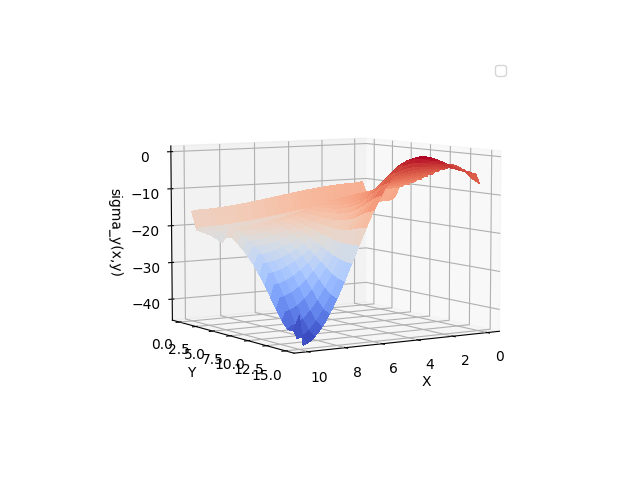
\includegraphics[width=0.49\textwidth, scale=1]{images/results/static_2/sigma_y_1.png}
        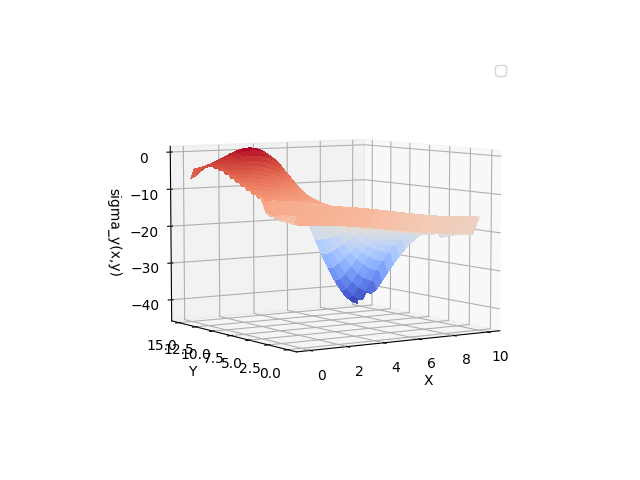
\includegraphics[width=0.49\textwidth, scale=1]{images/results/static_2/sigma_y_2.png}
        \caption{Функція $\sigma_y(x, y)$}\label{static_2_sigma_y_1}
    \end{center}
\end{figure}

\subsection{Висновки до треттього розділу розділу}
Отримано точне розв'язок статичної задачі для прямокутної області за другої основної задачі теорії пружності на бічних гранях.
Дослідженно поля переміщень та напружень для різних видів навантаження і розмірів прямокутної області.